%%%%%%%%%%%%%%%%%%%%%%%%%%%%%%%%%%%%%%%%%%%%%%%%%%%%%%%%%%
\section{Formalizing the technique}
\label{sec:formalizing}
%%%%%%%%%%%%%%%%%%%%%%%%%%%%%%%%%%%%%%%%%%%%%%%%%%%%%%%%%%

This section defines the formalisms used by InvariMint, explains the process
used to construct a model equivalent to Synoptic's initial model, and provides
implementation details describing how InvariMint generates a final
model.

%The formal languages approach seeks to circumvent Synoptic's costly refinement and
%coarsening steps by generating a minimal deterministic finite
%automaton (DFA) that accepts the
%intersection of the
%language accepted by the initial Synoptic model and the languages accepted by
%DFAs corresponding to each of the mined invariants.

%%%%%%%%%%%%%%%%%%%%%%%%%%%%%%%%%%%%%%%%%%%%%%%%%%%%%%%%%%
\subsection{Definitions}
\label{sec:Definitions}
%%%%%%%%%%%%%%%%%%%%%%%%%%%%%%%%%%%%%%%%%%%%%%%%%%%%%%%%%%
\begin{definition} [Deterministic Finite Automaton]
A finite state machine that accepts or rejects finite strings of symbols. The
strings for DFAs described in this paper are traces of executions using log
events as symbols. Each DFA is defined by a finite set of states $S$, a finite
alphabet of log event types $\Sigma$, a transition function $\delta : S \times
\Sigma \rightarrow S$, an initial state $I \in S$, and a set of accept states
$F \subseteq S$.
\end{definition}

\begin{definition}[DFA Language]
For a DFA $D$ let $L(D)$ denote the language accepted 
by $D$. This describes the set of traces accepted by $D$. 
\end{definition}

\begin{definition}[Initial Model]
For a set of input traces $T$, consider the initial model
$M_i$ to be exactly the initial model used by Synoptic as described in
Section~\ref{sec:synoptic}. By
construction, $L(M_i) \supseteq T$, and $M_i$ is deterministic (as
there is exactly one node per event type). 
\end{definition}

\begin{definition}[Invariant DFA]
Let $i_1, \ldots, i_m$ be 
the set of invariants true over $T$.
For each invariant $i_j$, let $I_j$ be the corresponding DFA. 
Figure~\ref{fig:invRegDfa} illustrates how we translate each type of mined invariant
into a corresponding DFA. 
\end{definition}

\begin{definition}[DFA Intersection]
DFA intersection combines two DFAs $A_1$ and $A_2$ such that the resulting DFA $A$ will
accept a trace if and only if it is accepted by both $A_1$ and $A_2$.

Let $A_1=(S_1,\Sigma,\delta_1,I_1,F_1)$ and
$A_2=(S_2,\Sigma,\delta_2,I_2,F_2)$ be two DFAs.
We define the intersection $A$ of $A_1$ and $A_2$, written $A_1\cap A_2$, as the quituple
$$(S,\Sigma,\delta,I,F):=(S_1\times S_2,\Sigma,\delta, I_1\times I_2, F_1\times F_2),$$
where $\delta$ is a function
given by $$\delta((s_1,s_2),\alpha)=\delta_1(s_1,\alpha)\times \delta_2(s_2,\alpha).$$

$A$ can be thought of as a machine that runs
$A_1$ and $A_2$ simultaneously. A symbol $\alpha$ being fed into $A$ at start state $(q_1,q_2)\in I$
is the same as $A_1$ reading $\alpha$ at state $q_1$ and $A_2$ reading $\alpha$ at state $q_2$. The
set of all possible next states for the configuration $((s_1,s_2),\alpha)$ in $A$ is the same as the
set of all possible combinations $(t_1,t_2)$, where $t_1$ is a next state for the configuration
$(s_1,\alpha)$ in $A_1$ and $t_2$ is a next state for the configuration $(s_2,\alpha)$ in $A_2$.
\end{definition}

\begin{definition}[DFA Minimization]
Hopcroft's DFA minimization~\cite{hopcroft_minimization_tr1971} 
reduces a DFA, $A$, to the smallest possible DFA
preserving the language of $A$.
To do this, states in $A$ that are
behaviorally equivalent, or take the same action on all inputs, are grouped into
a set that corresponds to a single state in the final minimized model.

%Initially all states in $I$
%are split into 2 sets of accepting versus non-accepting states. The algorithm then
%iteratively loops over each set and each possible input symbol, splitting states
%that do not produce the same behavior for the given symbol. This 
%terminates once additional splits cannot be found.
\end{definition}

%%%%%%%%%%%%%%%%%%%%%%%%%%%%%%%%%%%%%%%%%%%%%%%%%%%%%%%%%%
\subsection{Constructing the initial model}
%%%%%%%%%%%%%%%%%%%%%%%%%%%%%%%%%%%%%%%%%%%%%%%%%%%%%%%%%%
The Synoptic model is not equivalent to the intersection of all the mined
invariants. Synoptic's initial model is constructed by merging the input traces in such a
way that if an event $x$ is ever immediately followed by an event $y$ in some input trace
then there is an edge between $x$ and $y$ in the model. Likewise
if $x$ is never immediately followed by $y$ across all input traces
then there is no edge between $x$ and $y$ in the initial model.

The initial model thus encodes a set of "can/cannot be immediately
followed by" properties that are not explicitly expressed with Synoptic's 
mined invariants but are instead the result of using the Synoptic process.
To capture those implicit properties, InvariMint expresses those properties as
invariants as well. For two event types $x$ and $y$, either $x$ can be
immediately followed by $y$, written $x~CIFby~y$, or $x$ is never immediately
followed by $y$, written $x~NIFby~y$.

$NIFby$ and the mined invariants
provide truth values that apply to every trace whereas
$CIFby$ is a special kind of invariant that describes a global property of
\emph{all} input traces. $x~CIFby~y$ means that in some traces it is possible
for $x$ to
be immediately followed by $y$ but says nothing about whether this will be the
case in an arbitrary trace.
These cannot be translated into useful DFA invariants: beginning with an
overly general model, InvariMint generates a more descriptive model
by intersecting the model with invariants that
constrain the behavior of each individual trace.

\newcommand\XOR{\mathbin{\char`\^}}
However for two event types $x$ and $y$, either $x~CIFby~y$ or $x~NIFby~y$ will be mined
from the input traces. Because of this relationship, the intersection of
all $NIFby$ invariants is sufficient for encoding all can/cannot be immediately
followed invariants. $x~NIFby~y$ is translated to a DFA using the regular
expression $([\XOR x]|xx^*[\XOR xy])^*x^*$.

We must also introduce an $Initial...Terminal$ invariant describing
the property that every trace must begin with a synthetic initial event and
terminate with a synthetic terminal event. This is necessary for InvariMint to
fully express the notion of traces with
clearly defined start and end points that is implicit in Synoptic models.
The initial and terminal events are
added to the input traces used by the invariant miner. This ensures that the temporal
relationships between these synthetic events and all other log events are
captured in the set of mined invariants. 

The initial InvariMint model is thus defined as the
intersection of languages accepted by these invariants. That is:\\

$M_i = \textrm{NIFby}_1 \cap ... \cap \textrm{NIFby}_n \cap
\textrm{$Initial...Terminal$}$\\

The language of InvariMint's initial model is equivalent to the language of
Synoptic's corresponding initial model.

\begin{figure}[t!]
   \center
   {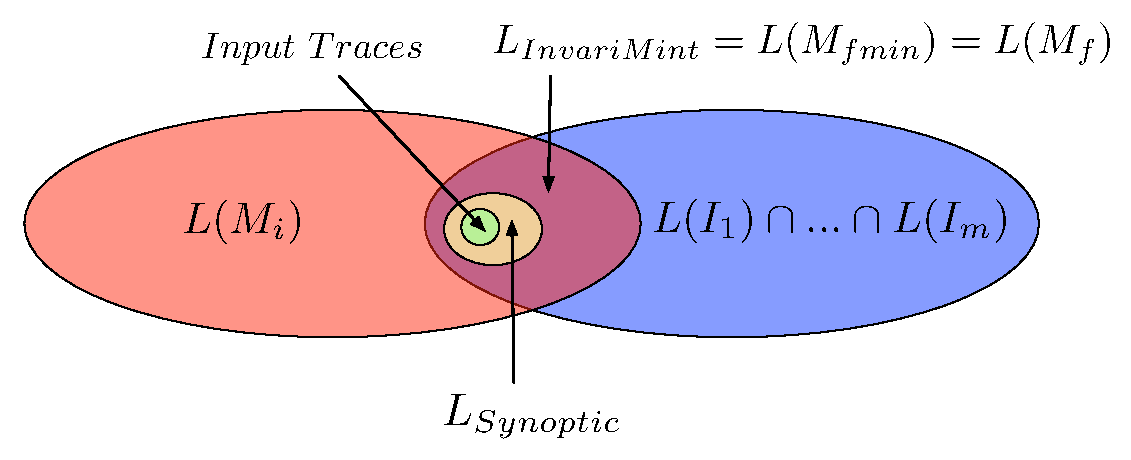
\includegraphics[width=0.95\columnwidth]{fig/language-venn.pdf}}
   \caption{This diagram illustrates the relationships between languages
    accepted by various models of the input traces. $L(M_i)$ is the language of
    the initial model which includes all of the input traces and is constrained
    only by the $NIFby$ invariants.
    $L(I_1) \cap \ldots \cap L(I_m)$ is the language of the intersected mined
    invariants. By design, $L(I_1)$ accepts all of the input traces.
    $L_{Synoptic}$ also accepts all of the input traces and is constrained by
    both the mined invariants and $M_i$. 
    Since Synoptic is non-deterministic, $L_{Synoptic}$ may vary given the same
    inputs but always respects the above constraints.
    $L_{InvariMint}$ is precisely the intersection of $L(M_i)$ and $L(I_1) \cap
    \ldots \cap L(I_m)$.
   } 
   \label{fig:language-venn}
\end{figure}


%%%%%%%%%%%%%%%%%%%%%%%%%%%%%%%%%%%%%%%%%%%%%%%%%%%%%%%%%%
\subsection{Constructing the final model}
%%%%%%%%%%%%%%%%%%%%%%%%%%%%%%%%%%%%%%%%%%%%%%%%%%%%%%%%%%
Define the DFA $M_f$ as the intersection $M_i \cap I_1 \cap \ldots
\cap I_m$ where $M_i$ is the initial model and $I_1, \ldots, I_m$
correspond to the set of mined
invariants defined in Section~\ref{sec:synoptic}.
By using the same invariants as Synoptic, we can both quantitatively and qualitatively
evaluate differences between models produced by the two techniques.

The corresponding language
$L(M_f)$ consists of all traces that
satisfy all of the mined and immediate invariants.  This language is generative
--- it includes $T$, the input traces, as well as all possible
stitchings of traces that satisfy the invariants. These stitchings are
possible traces allowed by the invariants but not yet observed in any input log.
Such traces are called synthetic traces, and exist in both Synoptic and
InvariMint models. These traces predict likely
future system behavior.

Having formed $M_f$ we can apply Hopcroft's classic DFA minimization
algorithm to $M_f$ to derive
$M_{f min}$. This algorithm guarantees that $M_{f min}$ is the smallest possible
DFA that accepts the same language as $M_f$. Figure~\ref{fig:language-venn}
summarizes the above discussion, which captures the
relationships between the languages accepted by $M_{f min}$,
$M_f$, and the other DFAs.

%%%%%%%%%%%%%%%%%%%%%%%%%%%%%%%%%%%%%%%%%%%%%%%%%%%%%%%%%%
\subsection{Implementation}
\label{sec:implementation}
%%%%%%%%%%%%%%%%%%%%%%%%%%%%%%%%%%%%%%%%%%%%%%%%%%%%%%%%%%

InvariMint uses the same parsing and invariant mining code used by Synoptic as
well as additional mining code to extract the immediate invariants.

The state machines manipulated by InvariMint are implemented as a layer above
the dk brics automata library~\cite{automaton}. This library provides regular expression parsing for
converting invariants to DFAs, as well as intersection and minimization
implementations of the algorithms described in Section~\ref{sec:Definitions}.
Our implementation provides an abstraction between the unicode alphabet
used by dk brics and the EventTypes mined from the input logs.
